%  Robotics Text  by Jacob Rosen and Blake Hannaford
% (c) 2007  Jacob Rosen and Blake Hannaford
%

\chapter{Manipulator Dynamics}


This chapter studies the relationship of manipulator motion to the forces and torques applied to the joints of the manipulator.   Forces (especially pertinent to prismatic joints) and torques (rotary joints) are conceptually very similar because they are often thought of  ``causes" of motion.   However, their mathematics tend to be rather different.  Since many manipulators are a mix of prismatic and rotary joints, we have to treat lots of special cases.   A notation which partially simplifies this solution is a set of generalized joint coordinates $q$.  For example, if the third joint of a six axis manipulator is prismatic, we would have:

\[
q =
\bmat q_1\\q_2\\q_3\\q_4\\q_5\\q_6\emat =
\bmat \theta_1\\ \theta_2 \\ d_3 \\ \theta_4 \\ \theta_5 \\ \theta_6 \emat
\]
and

\[
\dot q =
\bmat \dot q_1\\ \dot q_2\\ \dot q_3\\ \dot q_4\\ \dot q_5\\\dot q_6\emat =
\bmat \dot\theta_1\\ \dot\theta_2 \\ \dot d_3 \\ \dot\theta_4 \\ \dot\theta_5 \\ \dot\theta_6 \emat
\]
etc.


\section{Problem Statement and Learning Objectives}
\input{includes/Prob_and_Obj_06.tex}




\section{Basic Gravity Compensation}

In this section we will solve a relatively simple dynamics problem, but one of great practical importance:  we will develop some equations to compute the torques in each robot joint due to gravity.

First, let's consider a simplified situation in which a rigid shaft in an arbitrary direction supports a point mass at a distance (Figure \ref{basicgravitytorque}).   Suppose a point mass, having mass, $m$, and located at point $P$, is rigidly connected to the shaft but offset at some distance from the shaft and subject to the force of gravity, $mg$.

\begin{figure}\centering
   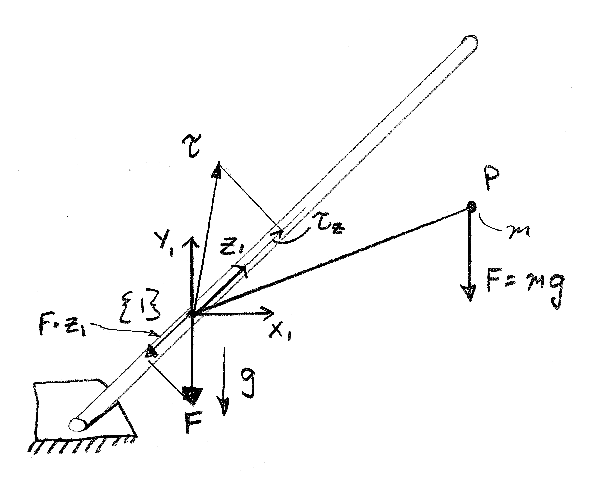
\includegraphics[width=3.5in]{figs06/00857.eps}
\caption{A shaft with an off-axis mass generating a torque and a force on the shaft.}\label{basicgravitytorque}
\end{figure}

Assume a frame, \{1\},  exists whose origin is on the shaft, and in which $Z_1$ is pointing along the shaft.  The moment generated about the origin of frame 1 is

\[
^1\tau =  P\otimes F = m(^1P \otimes ^1g)
\]
\[
^1\tau = m \begin{bmatrix} 0 & -Pz & P_y \\ P_z & 0 & -P_x \\ -P_y & P_x & 0  \end{bmatrix}
\begin{bmatrix} g_x\\g_y\\g_z \end{bmatrix} =
m\begin{bmatrix} P_yg_z-P_zg_y \\P_zg_x-P_xg_z\\P_xg_y-P_yg_x  \end{bmatrix}
\]
When we apply this to robot links, frame \{1\} will be the link frame and $Z_1$ will be the axis.  Thus the torque we are interested in is the $z$ component of $\tau$
\[
\begin{bmatrix}0\\0\\P_xg_y-P_yg_x\end{bmatrix}
\]

Now consider the force, $F=mg$ pointing ``down".  Besides the torque, the force, $F$, can also be represented in frame $\{1\}$, and it has a projection onto the $Z_1$ axis:
\[
F_z = F \cdot Z_1
\]




Applying this to a robot, we assume that the robot is not moving and that the joints are in some pose, $\theta$.

\begin{figure}\centering
   \includegraphics[width=3.5in]{figs06/00856.eps}
\caption{Two robot link frames ($i$, $i+1$) with centers of mass ($C_i$) and the gravity vector ($g$) shown for computation of gravity torques.}\label{linkcomstorque}
\end{figure}

Each link has mass, $m_i$ located at its center of mass: $C_i$ (Figure \ref{linkcomstorque}).
In link $i$, we wish to compute the $z$ component of torque due to the gravitational force on each center of mass which is more distal to the joint (has a greater subscript, $i$).
The moment on frame $i$ due to the mass in frame $j$ is therefore

\[
\tau_{ij} = C_j\otimes m_j g =  m_j ( C_j \otimes g)
\]
where we assume that all quantities are represented in the same frame.   For joint $i$, the natural frame is frame $\{i\}$:
\[
^i\tau = \sum_{j=i,n} m_j ({^iC_j} \otimes\; {^ig})
\]
\[
= \left [ \sum_{j=i,n} m_j {^iC_j} \right ] \otimes\;  {^ig}
\]

The quantity

\[
{C_{mi}} =  \sum_{j=i,n} m_j {C_j}
\]
is called the {\it first moment of mass} which is the center of mass times the total mass for the entire part of the manipulator distal to joint $i$ and it can be expressed in any frame in general.


The torque in the $i$'th joint, $\tau_i$ is therefore:

\[
\tau_i =  \hat{z}\cdot \;{^i\tau} = [0 \quad 0 \quad 1] \;{^i\tau} = \begin{bmatrix}0\\0\\{^i\tau_Z}\end{bmatrix}
\]
for rotary joints.



For prismatic joints,  we have the analogous equation
\[
F_{ij} = \sum_{j=i,n} m_j {^ig}
\]
and the joint force is just the $z$ component of $F_{ij}$.
\[
F_{Zi} =  \hat{z}\cdot F_{ij} = \begin{bmatrix}0\\0\\ F_{ijZ}\end{bmatrix}
\]


%%%%%%%%%%%%%%%%%%%%%%%%%%%%%%%%%%%%%%%%%%%%%%%%%%%%%%%%%%%%%%%%  Example with illustration
\begin{Example}
For the manipulator shown below, each $Z_i$ is shown in red and each center of mass is shown as a blue dot labeled with the total mass of each link, $m_i$.    The gravity vector is shown (drawn next to frame 0) to indicate its direction.


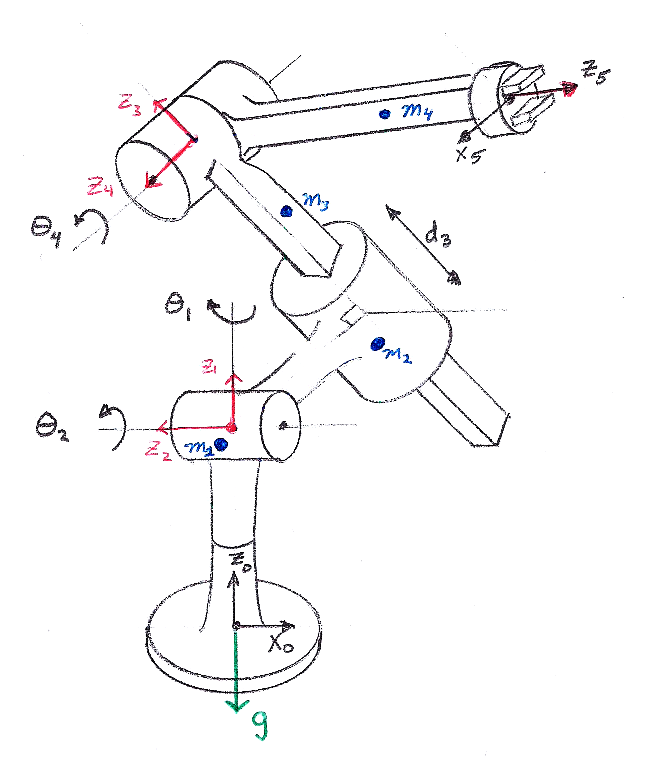
\includegraphics[width=80mm]{figs06/00695B.eps}

\subsection*{Part I}

Draw a vector on the diagram to illustrate each center of mass in the link's own frame:  $^iC_i$:

Draw the gravity force on each link.

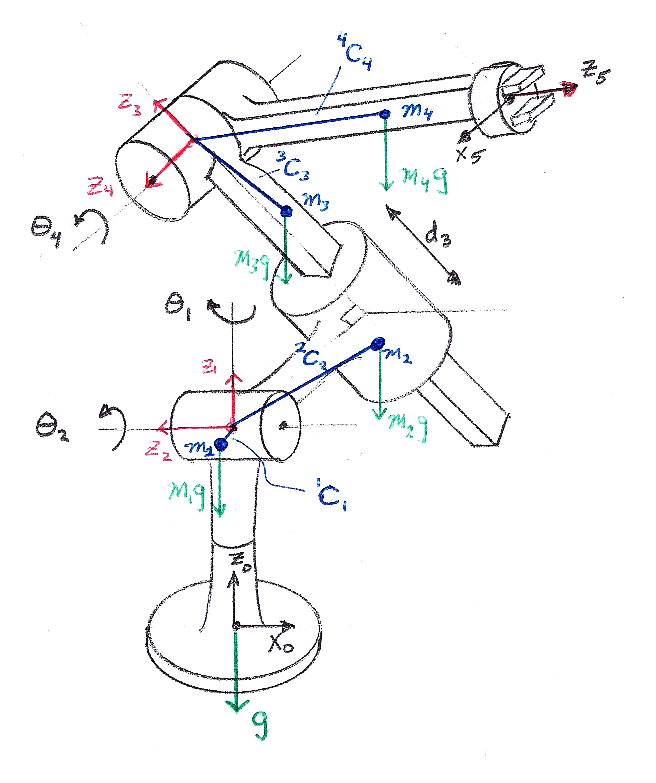
\includegraphics[width=80mm]{figs06/00858.eps}


\end{Example}
\begin{ExampleCont}

\subsection*{Part II}

Which masses contribute to torques on joint 2?

Draw a vector in place to illustrate each center of mass (that contributes to $\tau_2$) in   Frame 2:  $^2C_j$:

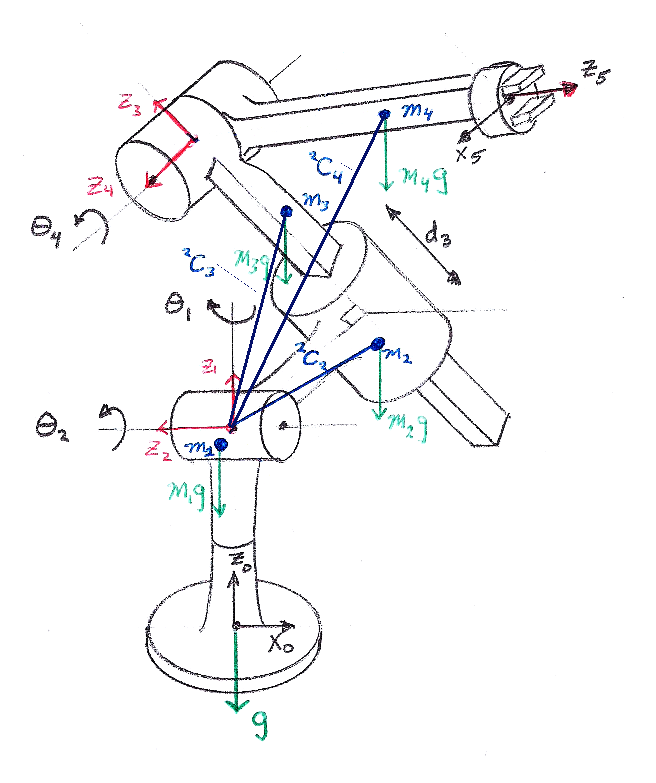
\includegraphics[width=80mm]{figs06/00858A.eps}





\end{ExampleCont}


%%%%%%%%%%%%%%%%%%%%%%%%%%%%%%%%%%%%%%%%%%%%%%%%%%%%%%%%%%%%%%%%%%%%%%%%%%%%%%%%%%%%%%%  example 1.1

\begin{ExampleSmall}
Derive the gravity torques for a three-link manipulator.  Joint 1 is rotary, Joint 2 is prismatic, joint 3 is rotary.  Assume that the robot is mounted on a level factory floor.
We know little about this manipulator, but we have obtained values for $m_j$ and ${^jC_j}$ and the ${^N_{N+1}T}$  matrices of forward kinematics (which depend on the robot pose of course).

\paragraph{Joint 1}
Transform the centers of mass,  $^jC_j$s into frame $\{1\}$:
\[
{^1C_3} = {^1_2T}\;{^2_3T}\;{^3C_3}
\]
\[
{^1C_2} = {^1_2T}\;{^2C_2}
\]
\[
{^1C_1} = {^1C_1}
\]
also because of the standard level floor mount:

\[
^0g = [ 0 \quad 0 \quad -9.8]^T
\]

now compute the acceleration of gravity in the current frame:

\[
{^1g} = \left [{^0_1R}^{-1} \right ] \; {^0g}
\]

Then we are ready:

\[
{^1\tau} = \left ( m_1{^1C_1}+m_2{^1C_2}+m_3{^1C_3}\right ) \otimes {^1g}
\]
Then the joint torque is
\[
\tau_1 = [0\quad0\quad1]\;{^1\tau}
\]

\paragraph{Joint 2}


\[
^2g =   {^1_2R^{-1}}\; {^0_1R^{-1}}\;{^0g}
\]
The gravity force vector arising from supporting the links distal to joint 2 is
\[
{^2F}= \left( m_2+m_3\right)\;{^2g}
\]
and the force on the prismatic joint is
\[
F_{Z2} =  [0\quad0\quad1]\;{^2F}
\]

\paragraph{Joint 3}
Joint three has torque only generated by its own weight.

\[
^3g =   {^2_3R^{-1}}\;{^1_2R^{-1}}\; {^0_1R^{-1}}\;{^0g}
\]

\[
^3\tau = m_3{^3C_3}\otimes {^3g}
\]

\[
\tau_3 = [0\quad0\quad1]\;{^3\tau}
\]


\end{ExampleSmall}



%%%%%%%%%%%%%%%%%%%%%%%%%%%%%%%%%%%%%%%%%%%%%%%%%%%%%%%%%%%%%%%%%%%%%%%%%%%%%%%%%%%%%%%%%%%%%%%%%%%%%%%%%%%%%%%%%%%%%%%%%%%%%%%%%%%%%%%%%%%%%%%%%%%%%%5
\section{Acceleration}

\subsection{Acceleration of a Particle}

A particle (point mass) moving in space is subject to acceleration when forces are applied to it according to
\[
F = m A
\]
where $A$ is a vector of the acceleration in three dimensions:
\[
A = \ddot{x} = [\ddot{X}, \ddot{Y}, \ddot{Z}]^T
\]

The particle may be subject to resistance due to viscous or damping forces such as friction or springs.   In this case these resistance forces, combined with $mA$ sum up to the applied force, $F$:
\[
F = mA + B\dot{x} + Kx
\]



\subsection{Acceleration of a Rigid Body}

A rigid body can be thought of as a collection of point masses which move together.
For linear motion, acceleration of a rigid body, measured at its center of mass, can be treated the same as that of a point mass.





\section{Equation of Motion of Rigid Bodies}
\subsection{Newton Equation}

Newton's equation is the fundamental equation of motion for linearly translating rigid bodies:

\[
\sum F = 0
\]
For example, a rigid body subject to an external force, $F$, having mass, $m$, and damping and elastic coefficients, $B, K$ respectively, would
have the equation of motion:
\[
0 = -F + mA + B\dot{x} + Kx
\]

\subsection{Euler Equations}

For rotation, each of the particles comprising a rigid body undergoes different motion.  The force acting on each particle is in general different.  However
the analogous concept of Moment or torque has been developed to predict rotational motion.   Moment, $M$, is an combination of force, $F$,  acting through a lever arm $\vec{r}$.
\[
M = F \otimes \vec{r}
\]
Where $\otimes$ stands for the vector cross product.
For a rotating body, Euler's equation of motion is
\[
\sum M = 0
\]
This analysis procedes similarly to linear motion, however the concept of mass must be generalized to an ``Inertia Tensor", $I$ (which will be explained in more detail below).
For example, a rigid body subject to a external moment, $M$, having  inertia tensor, $I$, and rotational damping and elastic coefficients, $B, K$ respectivly, would have the equation of motion:
\[
0 = -M + AI + B\dot{\theta} + K\theta
\]
where
\[
A = \ddot{\theta} = [\ddot{\theta_X}, \ddot{\theta_Y}, \ddot{\theta_Z}]^T
\]


\section{Inertia Tensor and Transformation of the Inertia Tensor}



\section{Derivation of the Inverse Dynamic Equations}
Fundamental to dynamic analysis of a manipulator is an answer to the question
\begin{quotation}
If a manipulator moves through the trajctory $\theta(t)$, what are the torques in each of its joints?
\end{quotation}


Goal:
$$
\tau = M(\theta)\ddot(\theta) + C(\theta, \dot{\theta}) + g(\theta)
$$


\section{Recursive Newton-Euler Formulation}
In this section, we will formulate the following problem:
\begin{quotation}
  Given the motion of a manipulator, specified in terms of the motion of it's joints, $q(t), \dot{q}(t), \ddot{q}(t)$, compute the torques in each joint, $\tau(t)$.
\end{quotation}




\subsection{Propagation of Acceleration}
From the previous chapter, we had
\[
^{N+1}\omega_{N+1} = \quad {^{N+1}_{N}R}\quad {^{N}\omega_{N}} +
\left[
\begin{array}{c}
0 \\
0 \\
\dot{\theta}_{N+1}
\end{array}
\right]
\]
and
\[
^{N+1}V_{N+1} =\quad  {^{N+1}_{N}R}\left[
   ^{N}V_{N} +
   ^N\omega_{N} \otimes \quad ^NP_{N,N+1}
   \right]
\]
for rotary joints, and
\[
^{N+1}\omega_{N+1} = \quad {^{N+1}_{N}R}\quad {^{N}\omega_{N}}
\]
\[
^{N+1}V_{N+1} =\quad  {^{N+1}_{N}R}\left[
   ^{N}V_{N} +
   ^{N}\omega_{N} \otimes ^NP_{N,N+1}
   \right] +
\left[
\begin{array}{c}
0 \\
0 \\
\dot{d}_{N+1}
\end{array}
\right]
\]
for prismatic.

If we combine them, but assume that only one of the pair $\{\dot\theta, \dot d\}$ is non-zero for any one joint, then


\[
^{N+1}\omega_{N+1} = \quad {^{N+1}_{N}R}\quad {^{N}\omega_{N}} +
\left[
\begin{array}{c}
0 \\
0 \\
\dot{\theta}_{N+1}
\end{array}
\right]
\]

\[
^{N+1}V_{N+1} =\quad  {^{N+1}_{N}R}\left[
   ^{N}V_{N} +
   ^{N}\omega_{N} \otimes ^NP_{N,N+1}
   \right] +
\left[
\begin{array}{c}
0 \\
0 \\
\dot{d}_{N+1}
\end{array}
\right]
\]

is one set of equations we can use for both types of joint.  For dynamics we need acceleration (Newton's equation) and angular acceleration (Euler's equation) so we need to differentiate these expressions.  There are terms in these equations of the form
\[
RV
\]
where $V$ is a vector and $R$ is a rotation matrix between the links.  Unfortunately, $R$ is changing with time since links can be rotating with respect to each other ($^i\omega_{i+1}\neq 0$). In Appendix \ref{derivativeofrotationmatrix},
 we take the derivative of this term, and apply the product rule and obtain
\[
\frac{d}{dt} R(t) = \dot{R}(t) = \omega\otimes
\]
In other words, if the rotation matrix is changing with time, there must be an angular velocity, $\omega$, and the equivalent of
the derivative of the rotation operator is $\omega\otimes$.

If we have the term
\[
f(t) = R(t) V(t)
\]
through the chain-rule its derivative is
\[
\frac{d}{dt} R(t)V(t) = R(t)\dot V(t) + \omega \otimes R(t) V(t)
\]
where $\omega$ is the angular velocity vector which represents the orientation change, and $\otimes$ designates the vector cross product.   Thus, to differentiate the angular velocity propagation expression, we have

\[
\frac{d}{dt}\:
{^{N+1}\omega_{N+1}} =
^{N+1}\dot\omega_{N+1} = ^{N+1}_NR\;^N\dot{\omega}_N + \dot{R}^N\omega_N + \bmat 0\\0\\\ddot\theta_{N+1}\emat
\]
\[
= {^{N+1}_{N}R}\quad {^{N}\dot\omega_{N}} + \; {^{N+1}\omega_N}\otimes\;{^{N+1}_NR}^N\omega_N+ \bmat 0\\0\\\ddot\theta_{N+1}\emat
\]
or
\bq
^{N+1}\dot\omega_{N+1} = ^{N+1}_NR \left [
  ^N\dot\omega_N + ^N\omega_N\otimes\bmat 0\\0\\\dot\theta_{N+1}\emat
\right] +
\bmat 0\\0\\\ddot\theta_{N+1}\emat
\eq

After we have computed all the $^N\omega_N$, we can do the linear acceleration.  We obtain the method by differentiating

\[
^{N+1}V_{N+1} =\quad  {^{N+1}_{N}R}\left[
   ^{N}V_{N} +
   ^{N}\omega_{N} \otimes ^NP_{N,N+1}
   \right] +
\left[
\begin{array}{c}
0 \\
0 \\
\dot{d}_{N+1}
\end{array}
\right]
\]

To perform this derivative, we will use the $\dot{R}$ result above, and also we will need a term of the form
\[
\frac{d}{dt} \; {^NP_{N,N+1}}
\]

To get this derivative we need to understand particular properties of ${^NP_{N,N+1}}$ which is the offset between Frame $N$ and frame $N+1$.  Let's look at how ${^NP_{N,N+1}}$ changes during a brief time interval $\Delta t$.   First, since link $N$ is a rigid body, and its angular velocity is $^N\omega_N$, we have a term which is a cross product of the two.   Second, if the link is prismatic, there is a change in the origin of Frame $N+1$ due to the sliding motion along $Z_{N+1}$, $\Delta Z_{N+1}$.   The sum of these terms is:

\[
\frac{d}{dt} \; {^NP_{N,N+1}}  = \;{^N\omega_N}\otimes \;{^NP_{N,N+1}} + \;{^N_{N+1}R}\bmat 0\\0\\\dot{d}_{N+1}\emat
\]
This situation is illustrated below

\begin{center}
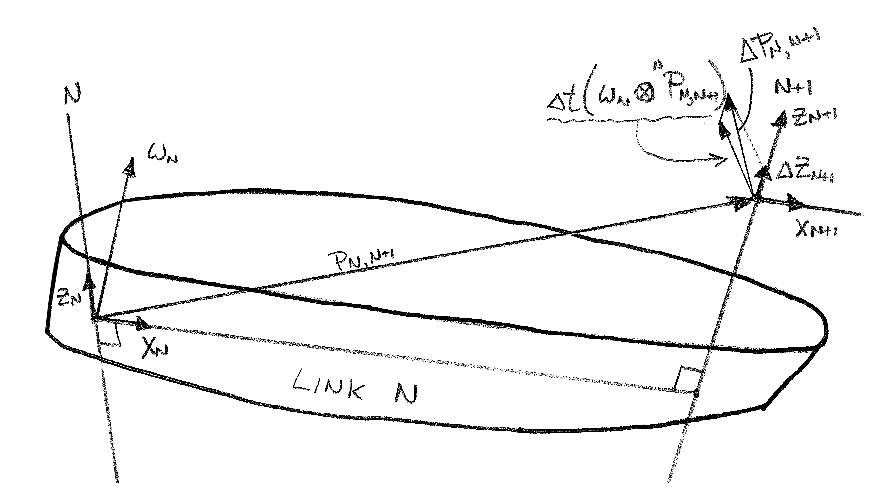
\includegraphics[width=120mm]{figs06/00918.eps}
\end{center}

[[ More derivation steps here ...]]

\bq
^{N+1}\dot V_{N+1} = {^{N+1}_NR}
\left [
   ^N\dot{\omega}_N\otimes \; {^NP_{N+1}} + \; {^N\omega_N} \otimes\; {^N\omega_N} \otimes\; {^NP_{N+1}} +\; {^N\dot V_{N}}
\right ]
+
2\:^{N+1}\omega_{N+1}\otimes\bmat0\\0\\\dot d_{N+1} \emat + \bmat0\\0\\\ddot d_{N+1} \emat
\eq
For rotary joints, the $\dot d, \ddot d$ terms are zero.

\subsubsection{Acceleration of the link mass center}
To get Newtonian reaction forces on each link, we need to derive the acceleration of the center of mass of each link.   We designate the Center of Mass of link N in frame N as
\[
^NP_{CN}
\]
Then the velocity of the center of mass is (see Section \ref{sectionrigidbodies} ) can be expressed by

\[
V_{CN} = V_N +\; \omega_N \otimes P_{CN}
\]
 (in any frame)

Differentiating this in frame $N$,

[[ More derivation steps ]]

\[
{^N\dot V_{CN}} = {^N \dot V_N}+\; {^N\dot\omega_N}\; \otimes \; {^NP_{CN}} + \; {^N\omega_N}\otimes \;  {^N\omega_N}\otimes\; {^NP_{CN}}
\]


\subsection{Propagation of Forces and Moments}
In this section $f_i$ will be the force applied to link $i$, and $m_i$ will be the moment applied to link $i$.

{\bf Step 1: } First we start with link $i$ at rest:

\includegraphics[width=4.0in]{figs06/00922.eps}

{\bf Step 2: } Now let
\begin{quotation}\noindent
$f_i = $ force on link $i$ by link $i-1$\\
$m_i = $ moment  on link $i$ by link $i-1$
\end{quotation}

{\bf Step 3: }
Add effects from link $i-1$:


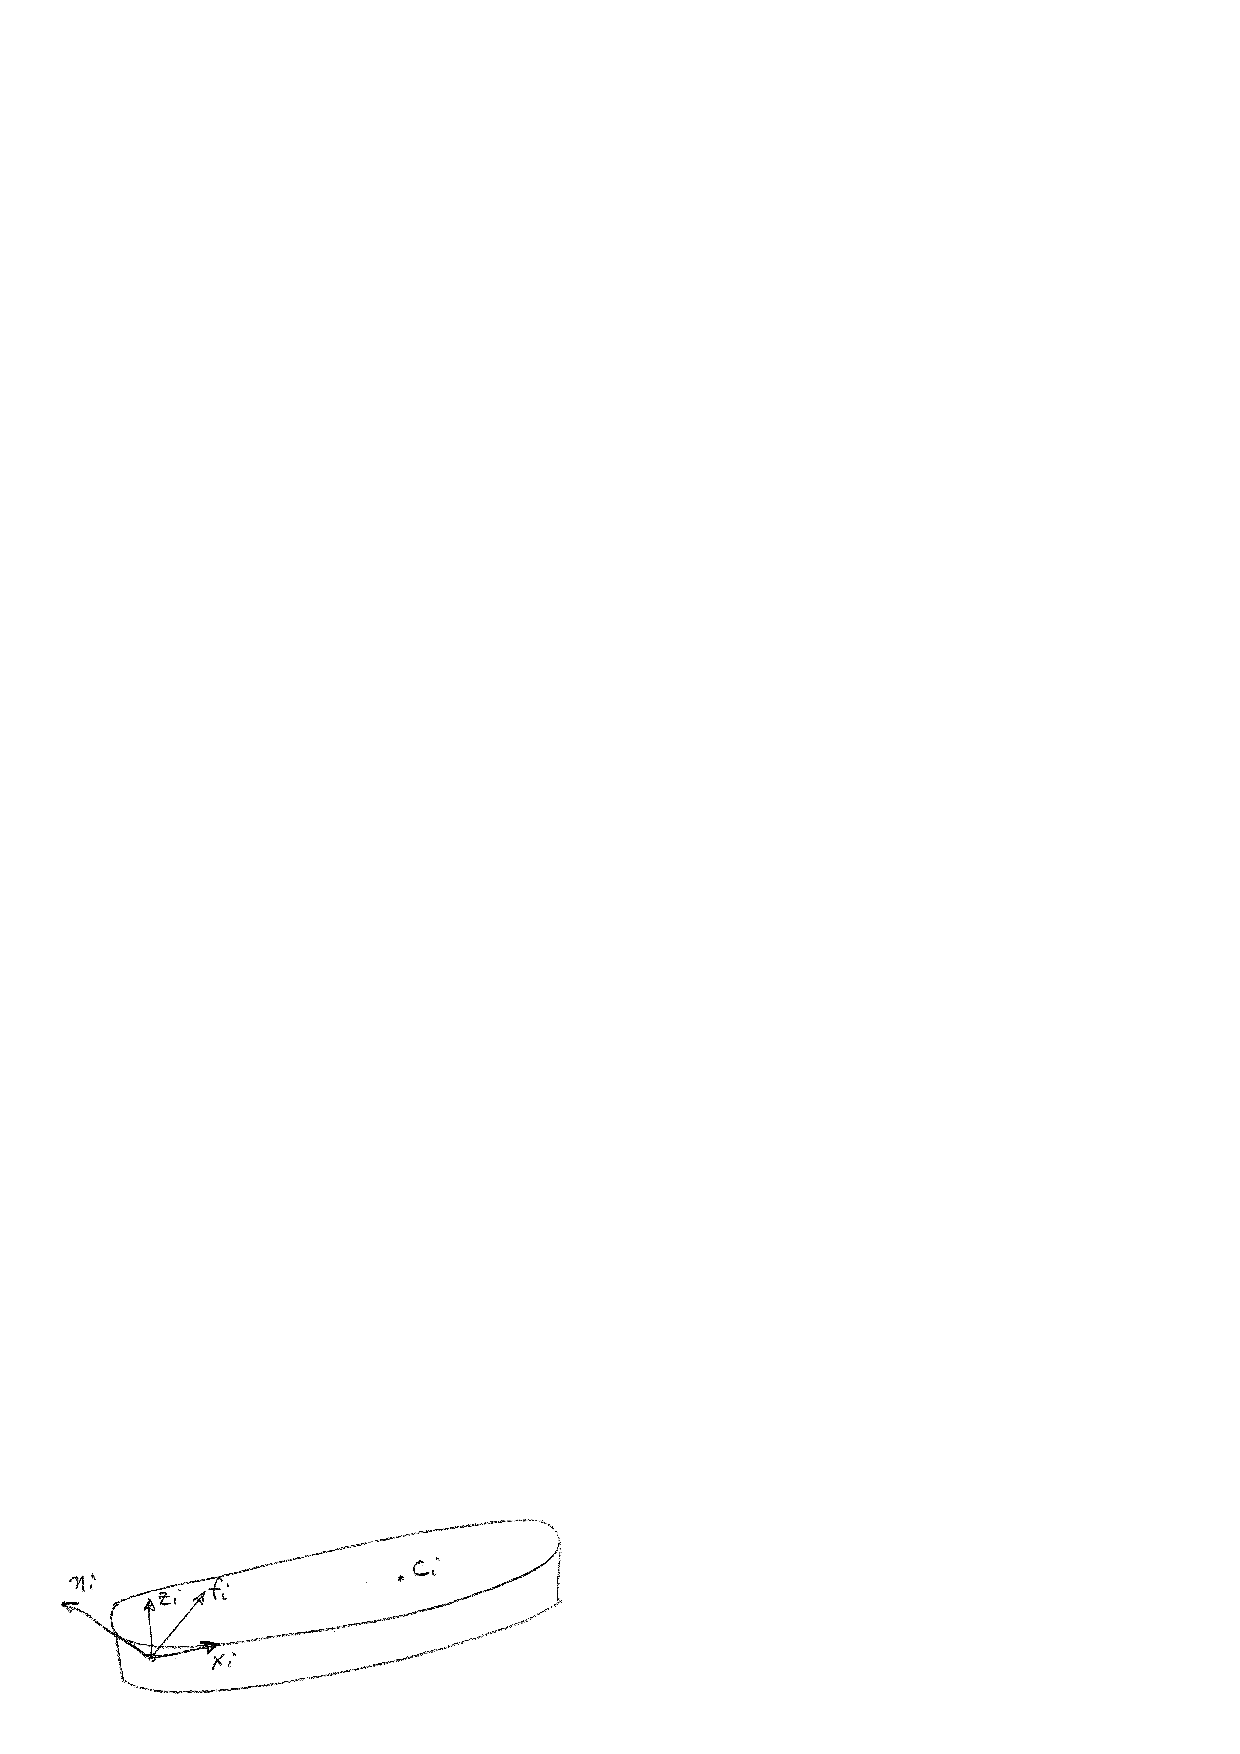
\includegraphics[width=4.0in]{figs06/00923.png}

(the figures use $n_i$ instead of $m_i$ -- this will be fixed!)


{\bf Step 4: }
Add in the effects from the next link, $i+1$:


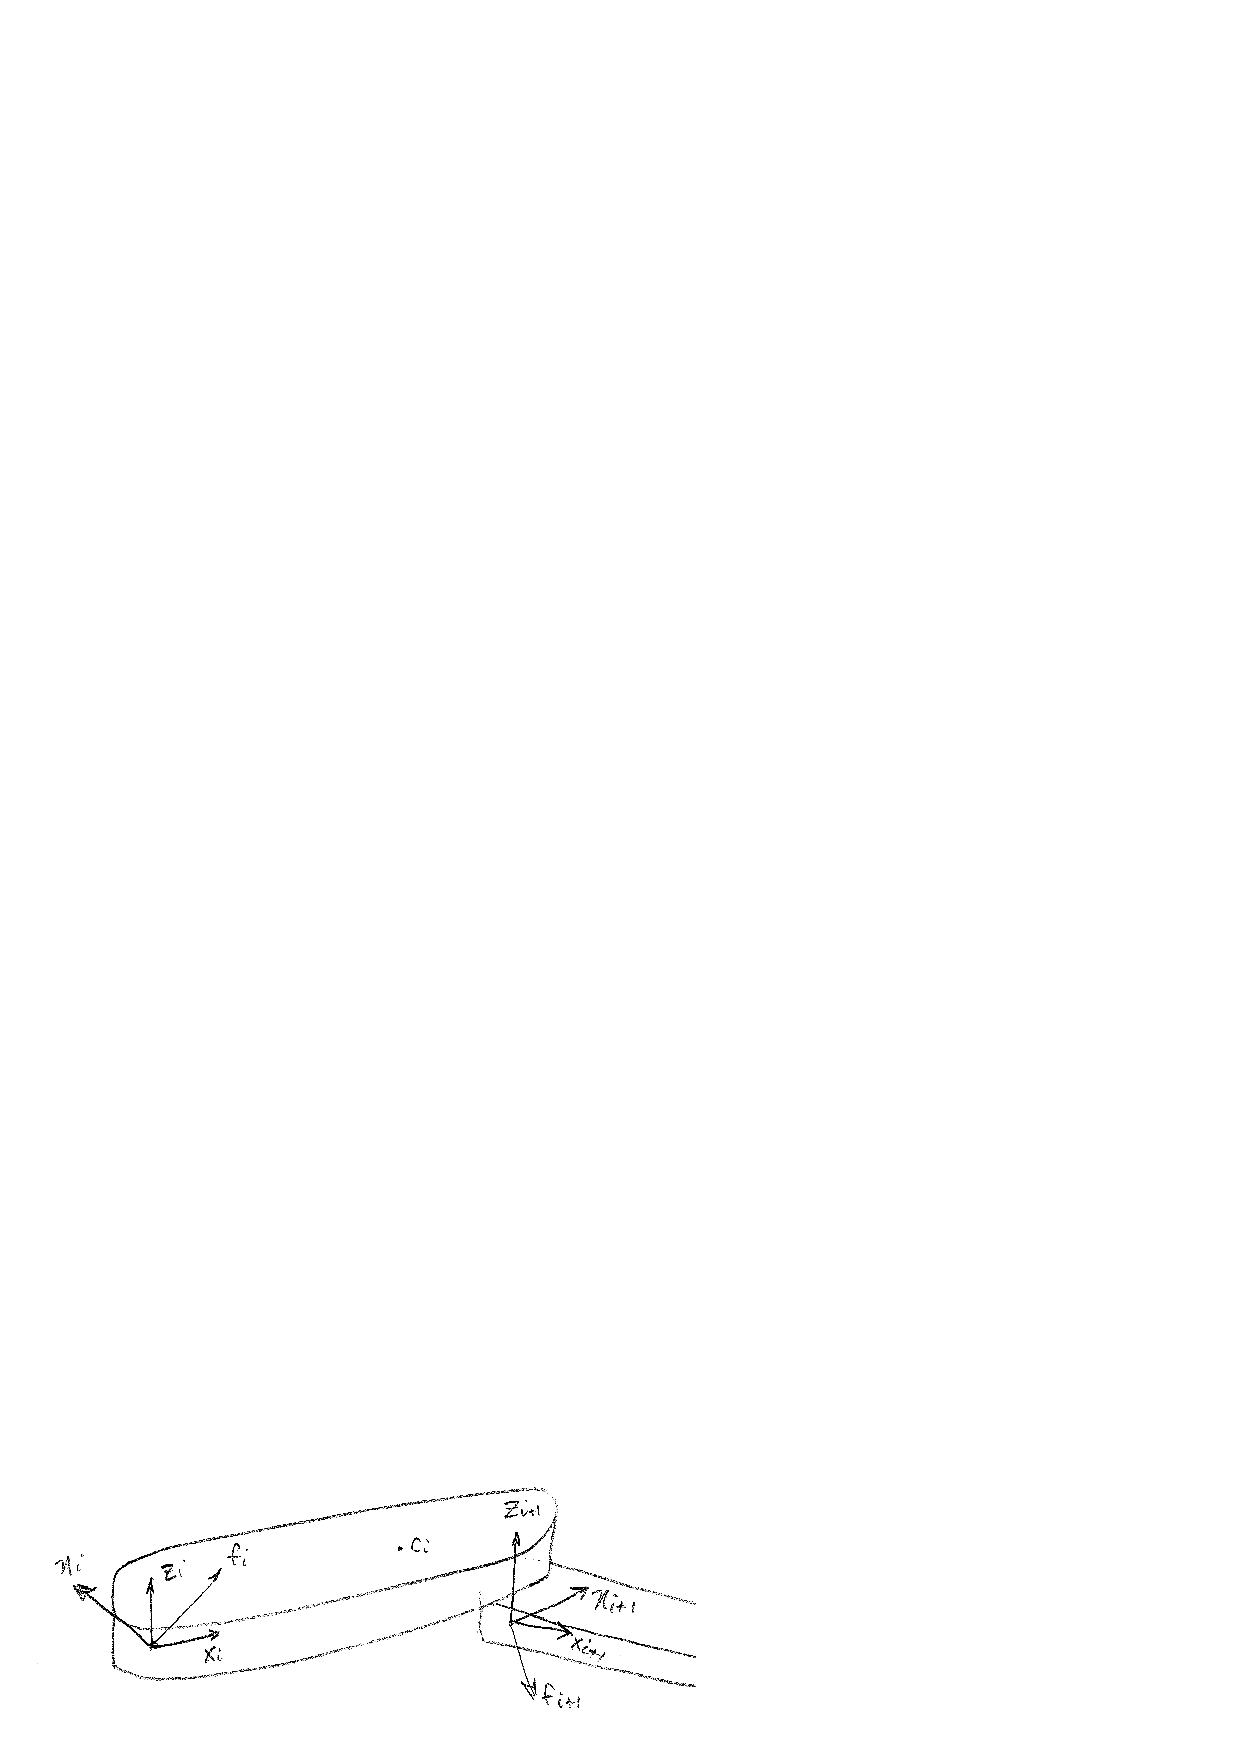
\includegraphics[width=4.0in]{figs06/00924.png}


{\bf Step 5: }
Balance forces and torques for static equilibrium in any frame
\[
f_i + f_{i+1} = 0
\]
Torque, unlike force, must be computed and balanced in a specific frame:
\[
m_i+n_{i+1}+P_{i,i+1}\otimes f_{i+1}
\]
We will also need this balance in the center of mass (COM) frame, which is an arbitrary point, $C_i$ on link $i$:


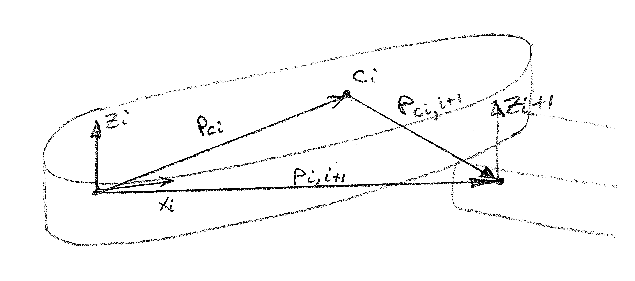
\includegraphics[width=4.0in]{figs06/00925.eps}

\[
m_i+n_{i+1}+(P_{Ci})\otimes f_i+(P_{ci,i+1})\otimes f_{i+1}
\]
where $P_{ci,i+1} = P_{i,i+1}-P_{Ci}$.


{\bf Step 6: }
Now we add in dynamic terms due to motion:
\[
F_i = m_i\dot{V}_i \qquad  \qquad N_i ={^CI}\dot{\omega}_i+\omega_i\otimes{^CI}\omega_i
\]
getting
\begin{equation}
f_i+f_{i+1} = F_i
\end{equation}
\begin{equation}
m_i+n_{i+1}+P_{Ci}\otimes f_i + (P_{i,i+1}-P_{Ci})\otimes f_{i+1} = N_i
\end{equation}

{\bf Step 7: } Rewriting the torque balance:
\[
m_i+n_{i+1}+P_{Ci}\otimes f_i + (P_{i,i+1})\otimes f_{i+1} - (P_{Ci})\otimes f_{i+1} = N_i
\]
\begin{equation}
m_i+n_{i+1}+P_{Ci}\otimes F_i + (P_{i,i+1})\otimes f_{i+1} = N_i
\end{equation}
where we have used
\[
P_{Ci}\otimes f_i - (P_{Ci})\otimes f_{i+1} = P_{Ci}\otimes (f_{i+1}+f_{i}) = P_{Ci}\otimes F_i
\]

{\bf Step 8: }
Now assume frame $i$ quantites are all known in frame $i$.  For example, $^{i+1}f_{i+1}$ is known.  Then we re-write the Force/Torque balance
\[
^if_i -  {^i_{i+1}R}\; {^{i+1}f_{i+1}} =  ^iF_i
\]
or
\begin{equation}
^if_i = ^iF_i + {^i_{i+1}R} \: {^{i+1}f_{i+1}}
\end{equation}
and similarly
\begin{equation}
^im_i = {^i_{i+1}R}\;{^{i+1}n_{i+1}}+{^iP_{Ci}} \otimes {^iF_i} + (^iP_{i,i+1})\otimes \left( {^i_{i+1}R}\;{^{i+1}f_{i+1}}\right) + {^iN_i}
\end{equation}

{\bf Step 9: }
Now, using Newton's and Euler's equations to get ${^iF_i}$ and ${^iN_i}$ for the last link and propagate downward.







\section{Lagrangian Formulation}
\section{Cartesian Transformation}


\section{Friction and Gravity Effects}

\section{Dynamic Simulation}


\subsection{Inverse Dynamics}
Computational Loads in Real Time Control

\section{Direct Dynamics}
Simulations

\section{Identification of Manipulator Dynamics}

\section{Summary of Notation}

% Summary of Notation for Chapter  06

